% ---------------------------------------------------------------------------
% Experiments section.
% Required packages: booktabs (\toprule/\midrule/\bottomrule/\cmidrule)
%                    amsmath  (\text in NFE$_\text{flow}$, \lVert \rVert)
% Everything else used here is core LaTeX. No color, multirow or siunitx.
% Dashes (--) mark experiments that are not run, or whose only available run is
% not budget-matched and is therefore not quotable.
% ---------------------------------------------------------------------------
\section{Experiments}
\label{sec:exp}

Our experiments ask three questions. Does a single-pass heteroscedastic
Student-t head (HT) reach the task performance of an iterative head at a
fraction of the inference cost (\S\ref{sec:exp:vla}--\S\ref{sec:exp:real})?
Does the advantage come from the robust likelihood rather than from the
single-pass parameterization itself (\S\ref{sec:exp:ablation})? And is the
multimodality that iterative heads are believed to capture actually present in
what they produce (\S\ref{sec:exp:modes})?

\subsection{Setup}
\label{sec:exp:setup}

\paragraph{Benchmarks.} We evaluate on three families. (i) Six
vision-language-action stacks: GR00T-N1.7 on RoboCasa GR1, on BridgeData
(WidowX) and on Fractal (Google Robot), OpenVLA-OFT and $\pi_{0.5}$ on LIBERO,
and Cosmos-Policy on LIBERO-10. (ii) RoboMimic, ten tasks in both state and
image observation modes, under three backbones. (iii) A real robot, on a
planar pushing task.

\paragraph{Protocol.} Within every row of every table, all arms share the
training recipe, data, optimizer, budget and evaluation harness, and differ
only in the action head. The one exception is the $\pi_{0.5}$ flow entry, which
is a published reference rather than a run of ours and is marked as such. Success rates are reported at the checkpoint each
benchmark's own reference recipe prescribes. On RoboMimic, where no single
checkpoint is prescribed, we report both the best checkpoint and the average
over the last five evaluations, since the first is optimistic and the second is
sensitive to late-training drift. Episode counts are given per table where they are
recorded; for RoboMimic the episodes per evaluation and the number of training
seeds were not logged, so its differences should be read as ordinal rather than
tested. Any cell whose only available run is not budget-matched to its row is
left blank rather than quoted, as are experiments we have not run.

\paragraph{The HT head.} On the VLA stacks HT uses the fixed prescription
$\nu = 4d$, where $d$ is the dimension of the action chunk, applied to every
stack without per-task tuning; \S\ref{sec:exp:ablation} reports the sensitivity
to $\nu$. The RoboMimic runs predate that prescription and use the earlier
setting $\nu = 2d$; the $\nu$ used for the real-robot arm was not recorded.
Values of $\nu$ are therefore not comparable across
Tables~\ref{tab:vla},~\ref{tab:robomimic} and~\ref{tab:real}.

% ---------------------------------------------------------------------------
\subsection{Vision-language-action benchmarks}
\label{sec:exp:vla}

\begin{table}[t]
\centering
\caption{Success rate (\%) on six VLA stacks. All arms in a row share data,
recipe, budget and evaluation harness and differ only in the action head. NFE
is the number of network evaluations per action chunk at inference. HT uses
$\nu = 4d$. OpenVLA-OFT ships no flow head; its public reference is an $L_1$
head, quoted separately. NFE$_\text{flow}$ for the three GR00T stacks is the
model default \texttt{num\_inference\_timesteps} $= 4$
(\texttt{gr00t/configs/model/gr00t\_n1d7.py}), the same sampler for every
embodiment. $^\dagger$ The $\pi_{0.5}$ flow entry is the published number, not a
run of ours; it is a reference rather than a budget-matched arm, and only that
row's MSE and HT cells share a protocol. Standard errors: $2.3$ points on the GR1 mean, about $6$ pooled on
WidowX, about $2$ on the Fractal mean, $0.35$ on the $\pi_{0.5}$ four-suite
average; not available for Cosmos-Policy. Blank cells are not run or not
budget-matched.}
\label{tab:vla}
\begin{tabular}{llrrrrr}
\toprule
Stack & Eval protocol & $d$ & NFE$_\text{flow}$ $\downarrow$ & Flow $\uparrow$ & MSE $\uparrow$ & HT (ours) $\uparrow$ \\
\midrule
GR00T GR1 (RoboCasa)        & 24 tasks $\times$ 20 ep   & 232 & 4  & 44.1 & 37.8 & \textbf{51.5} \\
GR00T WidowX (Bridge)       & 7 tasks $\times$ 50 ep    & 56  & 4  & 57.1 & --   & \textbf{67.4} \\
GR00T Google Robot (Fractal)& 6 tasks $\times$ 100 ep   & 56  & 4  & \textbf{67.3} & -- & 63.5 \\
OpenVLA-OFT (LIBERO, 4 suites)& 4 $\times$ 500 ep       & 56  & -- & --   & --   & 96.0 \\
$\pi_{0.5}$ (LIBERO, 4 suites)& 4 $\times$ 1000 ep      & 350 & 10 & 96.9$^\dagger$ & 96.8 & 96.6 \\
Cosmos-Policy (LIBERO-10)   & 10 tasks $\times$ 10 ep   & 160 & 30 & 96.0 & --   & 96.0 \\
\bottomrule
\end{tabular}
\end{table}

\paragraph{A single-pass head matches flow on four of the five stacks that have
a flow comparator.} Table~\ref{tab:vla} compares flow matching, plain regression
(MSE) and HT under identical training and evaluation. HT is ahead of flow by
$7.4$ points on GR1 and $10.3$ on WidowX, and within noise of it on $\pi_{0.5}$
($-0.3$) and Cosmos-Policy ($0.0$); Fractal is the fifth and is a loss, treated
below. OpenVLA-OFT ships no flow head and so enters no comparison here: against
its released $L_1$ reference of $97.1$, HT reaches $96.0$ over $2000$ episodes.
Each iterative baseline runs its full sampler, so the comparison does not favor
HT by shortening theirs.

\paragraph{The inference saving is real on three stacks and absent on a fourth.}
On GR1, WidowX and $\pi_{0.5}$, HT replaces a $4$-, $4$- and $10$-step sampler
with a single network evaluation while matching or beating it. Cosmos-Policy is the
exception and we do not claim a saving there: its action head is served through
the same $30$-step joint video-action sampler as the baseline, so HT changes the
objective without changing the inference cost.

\paragraph{Fractal is a counterexample, and the failure is task-structured.}
On Google Robot, flow reaches $67.3$ and HT $63.5$. The deficit is not spread
across tasks: HT is ahead on both free-space picking tasks ($+6$ each) and
behind on the articulated, contact-rich ones, losing $25$ points on
close-drawer alone. Both arms sit below the released reference ($72.5$), so the
absolute level is set by our training rather than by the head. We report this
stack as a negative result and return to it in the limitations.

\paragraph{Plain regression is not a substitute for either.} Where the MSE
column is filled, it separates sharply from both iterative and robust
single-pass heads on the harder stack ($37.8$ vs.\ $44.1$ and $51.5$ on GR1)
and separates from neither on the saturated one ($96.8$ vs.\ $96.9$ and
$96.6$ on $\pi_{0.5}$: a spread of $0.3$ points, below the $0.35$-point standard
error of that four-suite average, on a benchmark that is close to solved). Single-pass alone therefore does not explain the
result; the likelihood does.

% ---------------------------------------------------------------------------
\subsection{RoboMimic}
\label{sec:exp:robomimic}

\begin{table}[t]
\centering
\caption{RoboMimic: mean success over ten tasks, at the best checkpoint and
averaged over late checkpoints. Every entry is our own run under one protocol, across three backbones
and both observation modes. Straight Flow is a flow head trained to map noise to
data in one step, and Regression is a plain MSE head; both are single-pass
controls for HT. Straight Flow differs from Regression only in that its input
is Gaussian noise rather than zeros.}
\label{tab:robomimic}
\begin{tabular}{lcccc}
\toprule
& \multicolumn{2}{c}{State} & \multicolumn{2}{c}{Image} \\
\cmidrule(lr){2-3}\cmidrule(lr){4-5}
Head & best $\uparrow$ & late $\uparrow$ & best $\uparrow$ & late $\uparrow$ \\
\midrule
Flow (iterative)     & \textbf{0.886} & \textbf{0.824} & 0.834 & 0.782 \\
MIP (2 steps)        & 0.857 & 0.806 & 0.852 & 0.759 \\
Straight Flow (1 step)& 0.808 & 0.740 & 0.785 & 0.721 \\
Regression (1 step)  & 0.800 & 0.739 & 0.783 & 0.718 \\
HT, ours (1 step)    & 0.850 & 0.783 & \textbf{0.884} & \textbf{0.809} \\
\bottomrule
\end{tabular}
\end{table}

\paragraph{On RoboMimic the ordering depends on the observation mode.}
Table~\ref{tab:robomimic} reports all five heads under one harness, so unlike
comparisons against published numbers no protocol difference is folded into the
gaps. With image observations HT is the strongest head on both statistics
($0.884/0.809$ against flow's $0.834/0.782$). With state observations flow
leads ($0.886/0.824$ against $0.850/0.783$) and is ahead on eight of the ten
tasks. One caveat applies to the image column only: two Chi-Tf MIP cells
collapse late in training (best $0.82$ and $0.92$, late $0.21$ and $0.04$), and
their best-to-late drop alone contributes $0.0497$ of the $0.050$ by which HT
leads MIP on the late statistic. The HT-over-MIP late-average ordering should
therefore not be relied on; the best-checkpoint gap of $0.032$ and the
comparison against flow are unaffected.

\paragraph{The image-mode margin is carried by the two long-horizon tasks.}
Averaged over backbones, HT's image-mode advantage over flow is $+0.38$ and
$+0.07$ on the two transport variants and $+0.06$ on tool-hang, and between
$-0.06$ and $-0.01$ on the remaining seven tasks. (The assignment of the ph and
mh labels within each RoboMimic task pair is not independently verified in our
records, so we name the transport variants only as a pair.) The gain is therefore
concentrated where the horizon is long and the demonstrations are hardest to
fit, not distributed over the benchmark.

\paragraph{State-mode RoboMimic is where a robust head buys least.} HT is
within $0.01$ of plain regression on six of the ten state tasks, and most of the
separation between them ($0.783$ vs.\ $0.739$, a mean gap of $0.044$) comes from
two: one transport variant ($+0.167$) and tool-hang ($+0.190$) together account
for $0.036$, or $81\%$ of it, with push-T ($+0.063$) and the other transport
variant ($+0.030$) supplying the remainder. On the six tasks where the two heads agree, a robust
likelihood neither helps nor hurts; we report this as an observation and do not
have a residual measurement on these tasks that would explain it.

% ---------------------------------------------------------------------------
\subsection{Real robot}
\label{sec:exp:real}

\begin{table}[t]
\centering
\caption{Real-robot success rate (\%). Push-T is evaluated over 50 episodes
with the initial object pose randomized by $\pm 5$ in $x$ and $y$ (the unit of
the translation range was not recorded) and $\pm 30^\circ$ in yaw. Per-arm
binomial standard errors at $n = 50$ are $4.9$, $7.0$ and $4.6$ points; the
standard error of the flow-minus-HT difference is $6.7$ points if the two arms
were evaluated on independent draws. Whether the initial states were paired
across arms was not recorded; under pairing the standard error of the difference
depends on the correlation between the arms' per-episode outcomes and may be
either smaller or, if that correlation is negative, larger, so we treat it as
unknown. The number of
training seeds per arm was not recorded.}
\label{tab:real}
\begin{tabular}{lrrr}
\toprule
Task & Flow $\uparrow$ & MSE $\uparrow$ & HT (ours) $\uparrow$ \\
\midrule
Push-T   & 86 & 54 & \textbf{88} \\
Hang mug & -- & -- & -- \\
\bottomrule
\end{tabular}
\end{table}

\paragraph{On hardware the two single-pass heads separate by 34 points while
HT ties flow.} Table~\ref{tab:real} holds the inference budget fixed more
cleanly than any simulated row: flow and HT are $86$ and $88$, a
$2$-point difference against per-arm standard errors of $4.9$ and $4.6$, which
we read as a tie under any plausible pairing. Plain regression reaches $54$ with
exactly the same architecture, data and single forward pass as HT, a $34$-point
gap that is several times either arm's standard error. The two arms differ only
in their training objective, so the result is consistent with an objective
effect of that size; with the seed count and the pairing protocol unrecorded we
cannot put an interval on it or exclude a run-level contribution.

% ---------------------------------------------------------------------------
\subsection{Ablation: which loss}
\label{sec:exp:ablation}

\begin{table}[t]
\centering
\caption{Loss ablation on GR00T GR1: success rate (\%), all arms at the same 60k-step budget and
the same evaluation harness (24 tasks $\times$ 20 episodes, standard error
$2.3$ points). Simple Huber caps the chunk-residual norm at $2.5\times$ its
running median; heteroscedastic Huber applies the same cap to $\lVert r
\rVert/\sigma$ with a $d\log\sigma$ term. Blank cells are not run or not
budget-matched.}
\label{tab:ablation}
\begin{tabular}{llr}
\toprule
Loss & Scale model & SR (\%) $\uparrow$ \\
\midrule
$L_1$                                & none                & 17.2 \\
MSE                                  & none                & 37.8 \\
Huber (simple)                       & running median      & 37.4 \\
Huber (heteroscedastic)              & learned $\sigma$    & 40.7 \\
Flow matching (4 NFE)                & --                  & 44.1 \\
Student-t, homoscedastic             & fixed $\sigma$      & --   \\
Heteroscedastic Gaussian             & learned $\sigma$    & --   \\
\textbf{HT}, $\nu = 2d$              & learned $\sigma$    & 47.5 \\
\textbf{HT}, $\nu = 4d$ (ours)       & learned $\sigma$    & \textbf{51.5} \\
\bottomrule
\end{tabular}
\end{table}

\paragraph{The learned scale and the soft gate each add to the gain, in that
order.} Table~\ref{tab:ablation} separates the head's two ingredients, a scale
model and a redescending gate, by adding them one at a time. Clipping alone is
not enough: simple Huber ($37.4$) reproduces MSE ($37.8$). Normalizing the
residual by a learned $\sigma$ before clipping adds $3.3$ points over simple
Huber ($40.7$), and replacing the hard cap with the Student-t gate adds a
further $6.8$ to $10.8$ ($47.5$ at $\nu = 2d$, $51.5$ at $\nu = 4d$). Clipping alone therefore
changes nothing, while the scale and gate steps each add, the gate more than the
scale.
$L_1$ is far worse than any of them ($17.2$), which shows that
down-weighting large residuals is not by itself the useful ingredient; this arm
does not isolate why $L_1$ collapses, and we have not identified the
mechanism.

\paragraph{This ordering is not yet a decomposition.} Adding the ingredients in
one order bounds how much each contributes on top of the other, but it does not
isolate either: the two arms that would --- homoscedastic Student-t, a gate
without a learned scale, and heteroscedastic Gaussian, a scale without a gate
--- are not run at this budget. We therefore report the ordering and do not
attribute the gain to either component alone.

\paragraph{The single free parameter is not sensitive.} Moving $\nu$ from $2d$
to $4d$ changes GR1 by $4.0$ points and WidowX by $4.5$; across all stacks
where both were run the fixed $\nu = 4d$ prescription is at or within a few
points of the swept optimum, and we use it everywhere without per-task tuning.

\begin{table}[t]
\centering
\caption{Single-pass controls on RoboMimic: mean success over ten tasks and
three backbones (late-average). Straight Flow and Regression share HT's inference
cost and differ only in the objective.}
\label{tab:singlepass}
\begin{tabular}{lcc}
\toprule
Head (1 NFE) & State $\uparrow$ & Image $\uparrow$ \\
\midrule
Regression (MSE)  & 0.739 & 0.718 \\
Straight Flow     & 0.740 & 0.721 \\
HT (ours)         & \textbf{0.783} & \textbf{0.809} \\
\bottomrule
\end{tabular}
\end{table}

\paragraph{Among single-pass heads the objective is what separates them.}
Table~\ref{tab:singlepass} holds the inference budget fixed at one forward pass
across three backbones and both observation modes. Straight Flow's point
estimates are within $0.003$ of plain regression ($0.740$ vs.\ $0.739$ on state,
$0.721$ vs.\ $0.718$ on image), while HT is ahead of both by $0.04$ to $0.09$.
The two controls differ only in their input --- Straight Flow draws Gaussian
noise where Regression uses zeros --- so on this benchmark the stochastic input
that an iterative head relies on shows no measurable benefit once the sampler is
removed. We do not have the seed and episode counts to call the two equivalent,
only to say the gap between them is far smaller than either one's gap to HT.

% ---------------------------------------------------------------------------
\subsection{What do iterative heads actually sample?}
\label{sec:exp:modes}

\begin{table}[t]
\centering
\caption{Same-state sampling at the exact evaluation settings. GR1 and
$\pi_{0.5}$ use a $K{=}16$ probe plus a 3000-state extreme search with fresh
$K{=}32$ verification. WidowX uses a $K{=}8$ screen over 3000 Bridge states
and 1000 observations from its own rollouts; 100 uniformly sampled on-policy
states are then tested with independent $K{=}32$ axis discovery and $K{=}64$
confirmation. The probed HT checkpoints are the $\nu = 2d$ variants, not the
$\nu = 4d$ ones of Table~\ref{tab:vla}; every HT variant is deterministic.}
\label{tab:modes}
\begin{tabular}{llrrrl}
\toprule
Policy & Inference & Spread & Eff.\ rank & Separation & Content of the variance \\
\midrule
WidowX flow                     & 4 steps  & $1.258$ & 2.9 & 3.55 (null 3.09) & gripper timing; sparse arm-phase modes \\
GR1 flow                        & 4 steps  & $0.299$ & 3.1 & 2.85 & one mode $+$ noise; rare hand-event timing \\
$\pi_{0.5}$ flow                 & 10 steps & $0.924$ & 4.6 & 3.23 & one path; gripper-transition timing \\
Push-T MIP                      & 1 pass   & $3\times10^{-4}$ px & 1.0 & -- & none (numerical jitter) \\
Push-T HT (ours)                & 1 pass   & $3\times10^{-4}$ px & 1.0 & -- & none (numerical jitter) \\
GR1 HT (ours, $\nu = 2d$)        & 1 pass   & $0$ & -- & -- & none (deterministic) \\
$\pi_{0.5}$ HT (ours, $\nu = 2d$)& 1 pass   & $0$ & -- & -- & none (deterministic) \\
\bottomrule
\end{tabular}
\end{table}

\begin{table}[t]
\centering
\caption{Held-out density ablation after separating contact-state outputs.
For each state, PC1 is learned from samples disjoint from all evaluated draws;
one- and two-Gaussian densities are then compared by four-fold held-out log
likelihood. The GR1 rows use identical samples from the same 30 adversarial
states. $\widetilde{\Delta\ell}$ is the median 2G-minus-1G score in nats per
projected draw, so negative values favor one Gaussian component.}
\label{tab:continuous-density}
\small
\begin{tabular}{lrrr}
\toprule
Subspace & States & 1G $>$ 2G & $\widetilde{\Delta\ell}_{\rm 2G-1G}$ \\
\midrule
WidowX arm, no phase split & 90  & 53/90 & $-0.018$ \\
WidowX arm, local phase    & 10  & 0/10  & $+0.170$ \\
GR1 arm $+$ waist          & 30  & \textbf{29/30} & $\mathbf{-0.279}$ \\
GR1 articulated hands      & 30  & 14/30 & $+0.256$ \\
GR1 all 29 joints          & 30  & 14/30 & $+0.246$ \\
$\pi_{0.5}$ arm             & 36  & \textbf{32/36} & $\mathbf{-0.266}$ \\
\bottomrule
\end{tabular}
\end{table}

\paragraph{Contact-state outputs account for the apparent mixture structure.}
Table~\ref{tab:continuous-density} repeats the density comparison after
separating gripper and articulated-hand outputs from continuous body motion.
On the same 30 GR1 states selected to maximize full-action separation, a second
Gaussian improves held-out prediction in 16/30 states when the hands are
included but only 1/30 for arm and waist. Exact normality on the independent
PC1 is rejected in 26/30 hand or full-joint distributions but only 1/30 body
distributions. Although GR1 represents its hands as continuous joint targets,
their sampled statistics are discrete-like: the finger joints move together
between two narrow open/close configurations. Across the 15 confirmed hard
states, 348/480 chunks hold one configuration throughout the eight-step
horizon, 118 transition once, and only 14 flicker. The analogous arm-only
audit favors one Gaussian component in 32/36 adversarial $\pi_{0.5}$ states.
Thus the continuous body-action cloud is predictively single-component even
where the full action vector is not.

\paragraph{The continuous conditional mean is itself an executable action.}
Single-component density shape alone does not rule out an off-manifold average,
so we test the MSE target directly on WidowX. At 40 on-policy states (20 per
task), we estimate the six-channel arm mean from 64 same-observation draws,
restore the exact simulator state, and execute the mean for the four actions
used before replanning. Eight fresh sampled chunks define the reference outcome
cloud. The gripper is never averaged: every sampled-arm, mean-arm and
medoid-arm comparison receives the identical sampled gripper sequence. The
mean path lies within one radial reference RMS in 39/40 states for position and
40/40 for orientation, and outside the empirical 95\% reference-path envelope
in 0/40. Its median between/within ratio is $0.415$ in position and $0.382$ in
orientation, compared with $0.770$ and $0.575$ for the nearest sampled arm
medoid (paired one-sided Wilcoxon $p=6.5\times10^{-8}$ and
$2.0\times10^{-5}$). Thus averaging the continuous actions produces a central
motion rather than an invalid compromise between routes.

\paragraph{Most sampled variance is not a choice between high-level plans.}
Table~\ref{tab:modes} probes what the iterative heads produce at the
states they are trained on. At a typical GR1 state the separation
distribution coincides with the Gaussian null ($2.85$ against a null median of
$2.90$) and the dominant variance direction is unrelated to the temporal
derivative of the mean chunk ($|\cos|$ median $0.07$, equal to the
random-direction baseline $1/\sqrt{232} = 0.066$): the spread is undirected
noise around a single mode. Structure does appear at rare states --- the
3000-state search deep-verified $15$ of them beyond the null's maximum --- but
every one splits on a switch-like articulated-hand configuration, i.e.\ on
when an open/close event fires rather than on which body action to take.
On $\pi_{0.5}$ the structure that does exceed the null is real but is not a
second action --- at the most separated state, $12$ of $16$ samples issue the
gripper-close command at chunk step $46$ and $4$ at step $47$, while the arm
channels differ by $0.013$ RMS, less than half of one control step of motion.

\paragraph{WidowX contains modes, but they are local maneuver phases.}
The unbiased confirmation over 100 on-policy states finds 27 full-chunk
positives: 22 are explained by the gripper test and five by the arm test; one
additional arm positive is diluted in the full space. A descriptive audit of
the fitted density and raw chunks leaves three clearly resolved, arm-dominated
profiles. Two drawer states choose between executing a wrist rotation within
the current chunk and deferring it (up to $12.4^\circ$ yaw difference); one
eggplant state shifts the same lateral-motion pulse within the eight-step
horizon (up to $1.5$ cm). These are not numerical jitter, so the literal claim
that the action distribution is unimodal is false. The structure is strongly
task-dependent: all 22 gripper positives occur among the 44 eggplant states,
while none of the 56 drawer states passes the gripper test.

An independent adjacent-state probe nevertheless localizes the three profiles
to short windows. With 64 fresh samples at offsets
$\{-4,-2,-1,0,1,2,4\}$, the two drawer splits pass the pre-specified test only
at $\{-2,0,+1\}$ and $\{-1,0\}$, and the eggplant split at $\{0,+2\}$; all
have disappeared by offset $+4$. The modes are therefore a choice of when to
execute one local maneuver, rather than persistent routes to different targets.

\paragraph{Exact-state forks directly test the route interpretation.}
We fit modes only over the four actions executed before the next replan, then
screen 165 additional on-policy states and independently deep-test 66. Four
states pass the full criterion (fresh $K{=}32$ discovery and $K{=}64$
confirmation, $\Delta\mathrm{BIC}\geq10$, separation $\geq2$ pooled standard
deviations, component mass $\geq0.2$, and two resolved density peaks); all
remain significant after Bonferroni correction over both arm groups and every
adaptive deep test ($p=0.026$). At each state we restore the simulator and
controller exactly, execute 12 typical confirmation chunks from each
component, and then let the stochastic policy replan through 48 simulator
steps. Three modes induce a measurable initial pose split; the fourth is an
action-space split at which the arm does not measurably actuate.

The induced signal is a strong positive control: leave-one-branch-out mode
decoding from end-effector pose is $65/72$ during the forced prefix
($90.3\%$, 95\% Wilson interval $81.3$--$95.2\%$, permutation $p=0.0002$).
After replanning it falls to $40/72$ in the middle ($55.6\%$, $p=0.253$) and
$31/72$ late ($43.1\%$, $p=0.808$); the same pattern holds in each state
($83.3$--$95.8\%$ during intervention versus $29.2$--$50.0\%$ late). In every
motion-producing case, the late Euclidean distance between mode centroids is
only $0.24$--$0.35$ of the
radial within-mode RMS. No case has a significant late path, endpoint task
metric, or success split (all $p\geq0.53$, $0.10$, and $0.64$,
respectively). Thus, for these independently confirmed modes, the sampled
component causally changes the immediate maneuver but is not retained as a
closed-loop route variable.

\begin{figure*}[t]
  \centering
  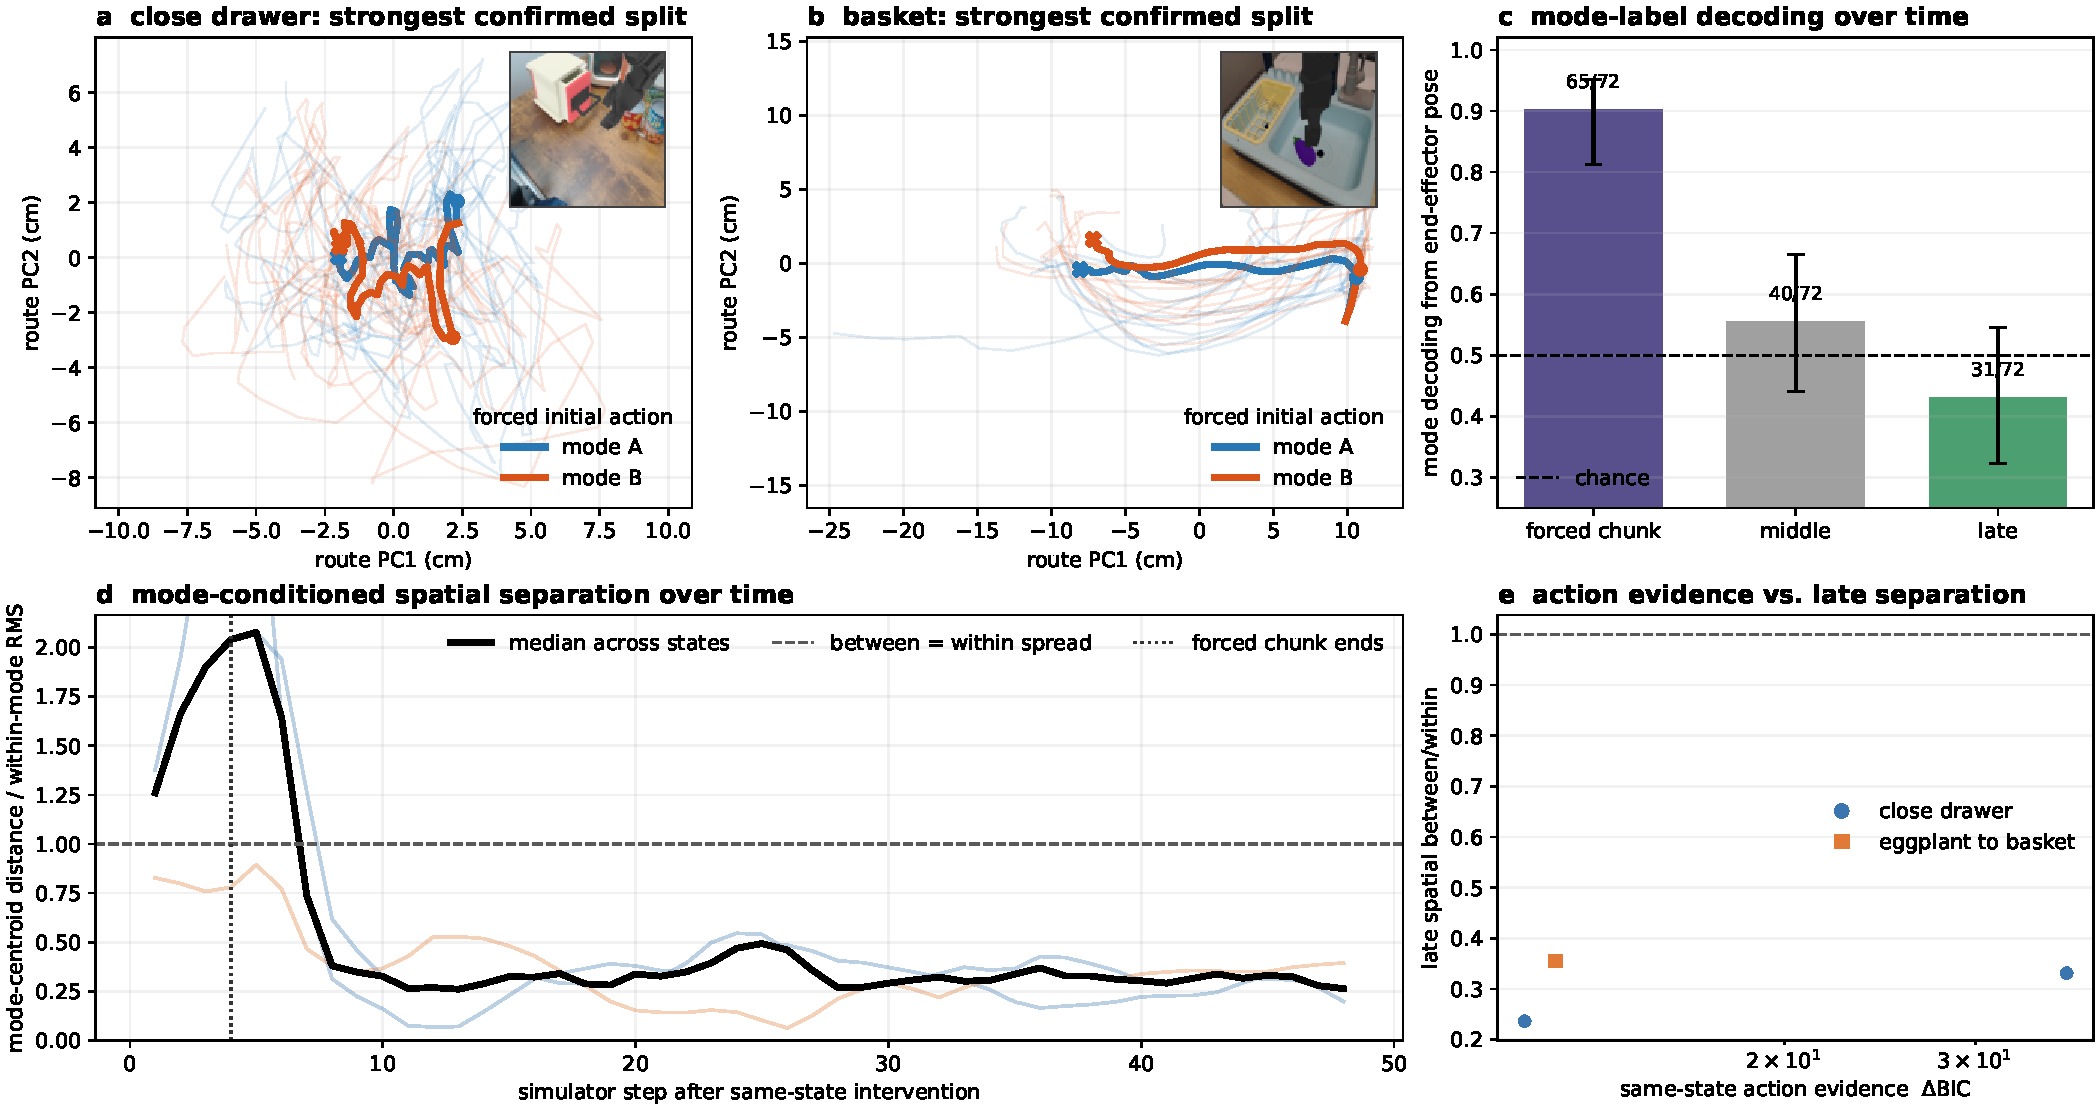
\includegraphics[width=\textwidth]{widowx_mm/widowx_branching_audit.pdf}
  \caption{\textbf{Same-state closed-loop forks of confirmed WidowX action
  modes.} Modes are fit only over the four actions executed before replanning.
  (a,b) Twenty-four branches from an identical state for a drawer and basket
  case, using 12 representative chunks per component; thin curves are
  individual end-effector paths, thick curves are component means, circles
  mark the end of the forced prefix, and crosses mark the final state after 48
  simulator steps. (c) Leave-one-branch-out mode decoding from full
  end-effector pose with Wilson 95\% intervals. (d) Euclidean distance between
  the two mode centroids divided by radial within-mode RMS; the vertical line
  marks the end of the intervention. (e) Independent action-space evidence
  does not predict persistent spatial separation. The fourth accepted mode is
  omitted from route aggregation because it produces no measurable arm
  actuation.}
  \label{fig:widowx-branches}
\end{figure*}

\paragraph{The iterative heads do not exhibit broad semantic-plan
multimodality.} Across GR1 and $\pi_{0.5}$, screening 3000 training states per
stack finds no alternative-action state: every above-chance case is undirected
noise or the timing of a discrete gripper/hand event. WidowX adds sparse arm
phase ambiguity, but its exact-state forks show that the tested components lose
their identity under closed-loop replanning. The supported statement is thus
not that large robot policies are mathematically unimodal, but that their
learned stochastic structure is dominated by event timing and local phase
rather than persistent high-level plan alternatives. Fractal and RoboMimic
flow heads remain unprobed;
OpenVLA-OFT has no flow head, and Cosmos-Policy is excluded because it generates
future video jointly with actions, making its seeded latent variance a different
object. Tables~\ref{tab:vla} and~\ref{tab:real} add the separate observation
that replacing these samplers with a deterministic head did not cost success.

% ---------------------------------------------------------------------------
\subsection{Limitations of the evaluation}
\label{sec:exp:limits}

\paragraph{HT is not uniformly better.} It loses to flow on Google Robot
($63.5$ vs.\ $67.3$) and on state-observation RoboMimic ($0.783$ vs.\ $0.824$),
and we do not currently have a criterion that predicts in advance which stacks
these will be. The positive results should be read as "matches or beats on most
stacks we tried", not as a guarantee.

\paragraph{The MSE comparison is thin.} The MSE column of
Table~\ref{tab:vla} is filled on two of six stacks. Three of the four blanks
(WidowX, Fractal, Cosmos-Policy) are experiments we did not run; the fourth,
OpenVLA-OFT, has an MSE run that is not budget-matched to its row and is left
blank rather than quoted. So within the VLA setting the claim that the robust
likelihood rather than the single forward pass carries the gain rests on GR1
alone: $\pi_{0.5}$ is a near-solved benchmark on which all three heads fall
within its $0.35$-point standard error, and on which fixed-$4d$ HT is in fact
$0.2$ below MSE, so it is a null comparison rather than supporting evidence. The
claim is carried elsewhere by RoboMimic and the real robot.

\paragraph{The loss ablation is reported only on GR1, and is incomplete there.}
Two of its arms --- homoscedastic Student-t and heteroscedastic Gaussian --- are
not run, so the section establishes an ordering along one chain
(MSE $\to$ Huber $\to$ heteroscedastic Huber $\to$ HT) and cannot isolate either
ingredient. No stack currently carries all five losses at a single budget.

\paragraph{Uncertainty is uneven across the tables.} Several cells are
single-seed. Where standard errors can be computed they are given in the
caption of the table that reports the number: Table~\ref{tab:vla} for the VLA
stacks, Table~\ref{tab:real} for the real robot, Table~\ref{tab:ablation} for
the GR1 ablation. For RoboMimic neither the episodes per evaluation nor the seed
count was recorded, so no RoboMimic difference in this section should be treated
as statistically established.
